\newcommand{\graphformatfig}{
\begin{figure}[h]
    \centering
    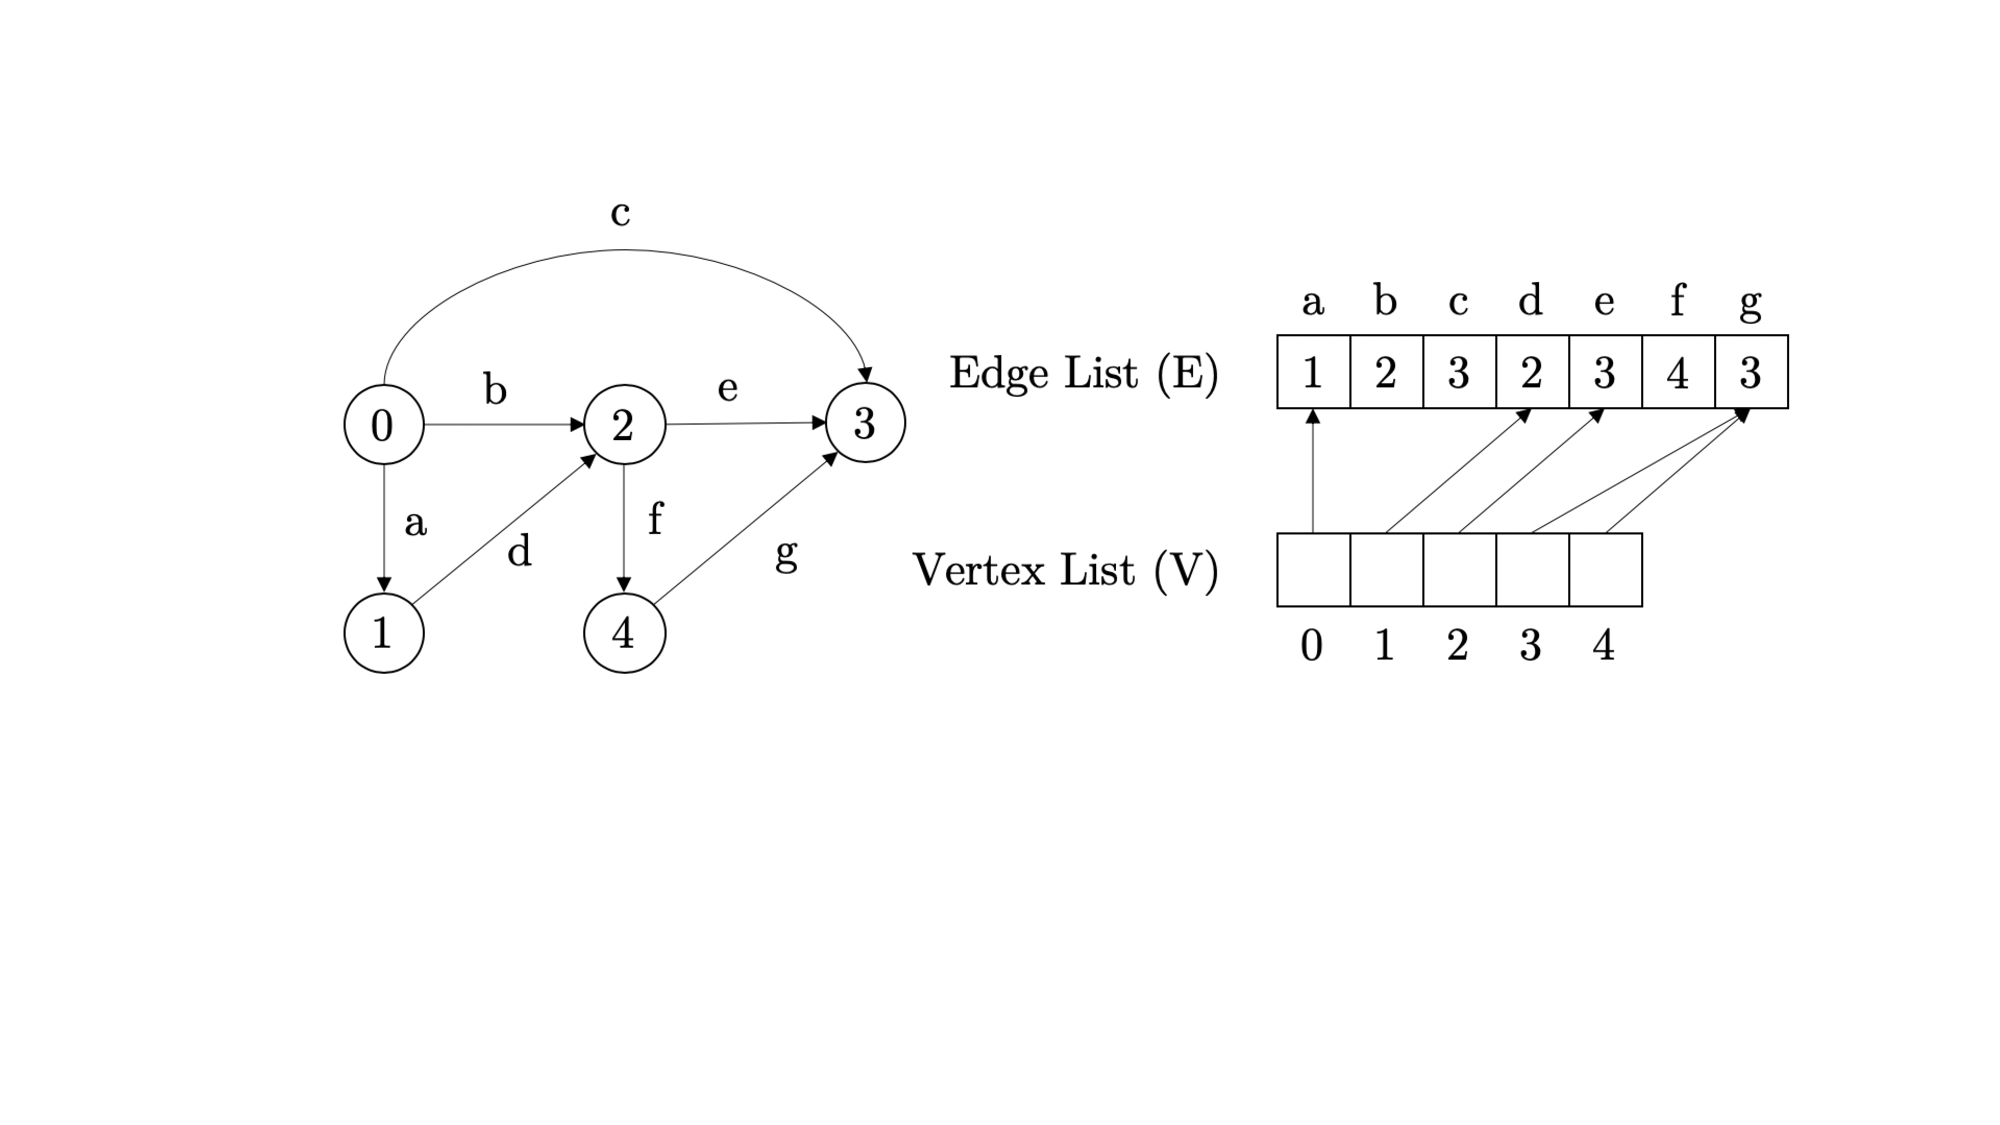
\includegraphics[width=0.8\textwidth]{graphit-figures/graph-format-figure.pdf}
    \caption{The CSR graph format that we use to store graph data on the manycore. For weighted graphs, the weight is stored with each element in the edge array.}
    \label{pap:generals2020:sec:background:fig:graphformat}
\end{figure}
}
\newcommand{\ugfoverview}{
\begin{figure}[t]
    \centering
    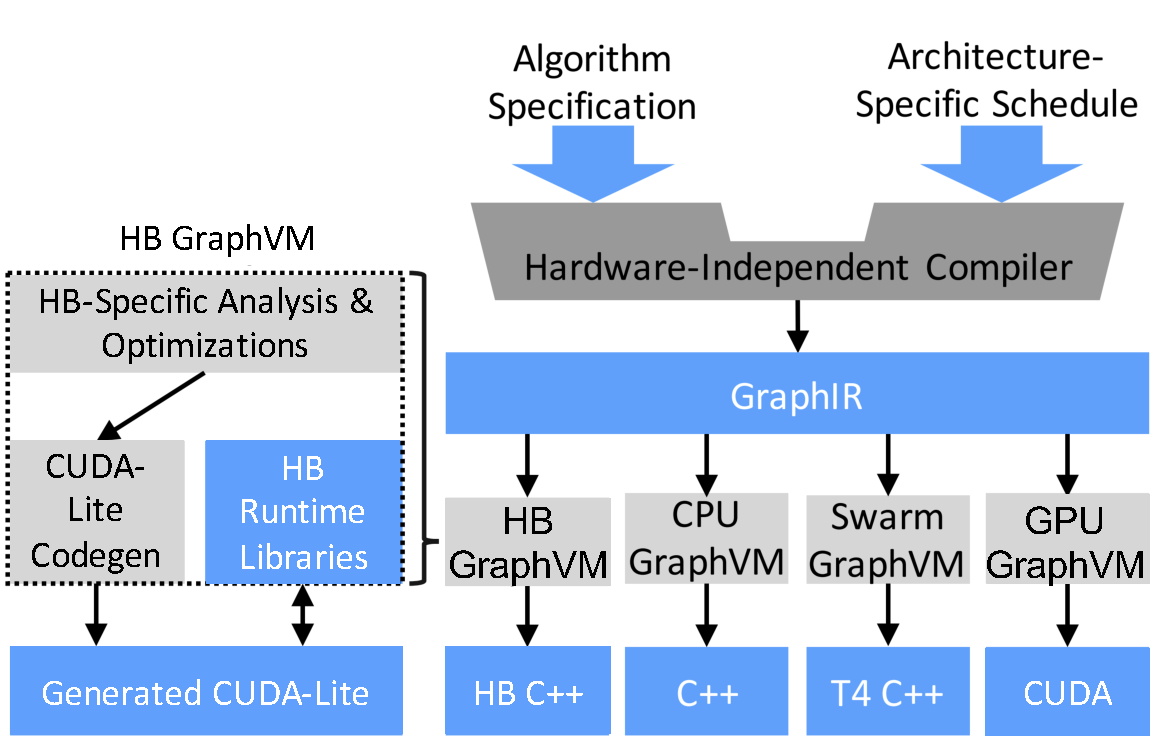
\includegraphics[width=0.8\textwidth]{graphit-figures/ugf.pdf}
    \caption{The \ugc (\GG). \graphisa decouples the hardware-independent part of the compiler from the hardware-dependent \graphvms. Grey blocks denote parts of the compiler, and blue blocks denote code (inputs, intermediates, libraries, or generated).}
    \label{fig:ugf}
\end{figure}
}